\selectlanguage{ngerman}
\subsection{App}\label{ch:Umsetzung_App}
% - Geschrieben mit Flutter und Dart
%   --> verschiedene Plattformen (Android, Windows, iOS, macOS, ...)
% - abonniert via MQTT die Topic (im Prototyp ist Topic hartkodiert; final Auswahl aus Liste, wenn allgemeine App)

Um die aktuelle Parkhausbelegung für den Nutzer darzustellen, wurde eine App entwickelt, die mithilfe von Flutter und Dart geschrieben wurde und daher verschiedene Plattformen, wie Android, Windows, iOS und macOS, bedient.
In Abbildung~\ref{fig:app} sind Screenshots der App dargestellt.

\begin{figure}[h]
	\centering
	\subfloat{
		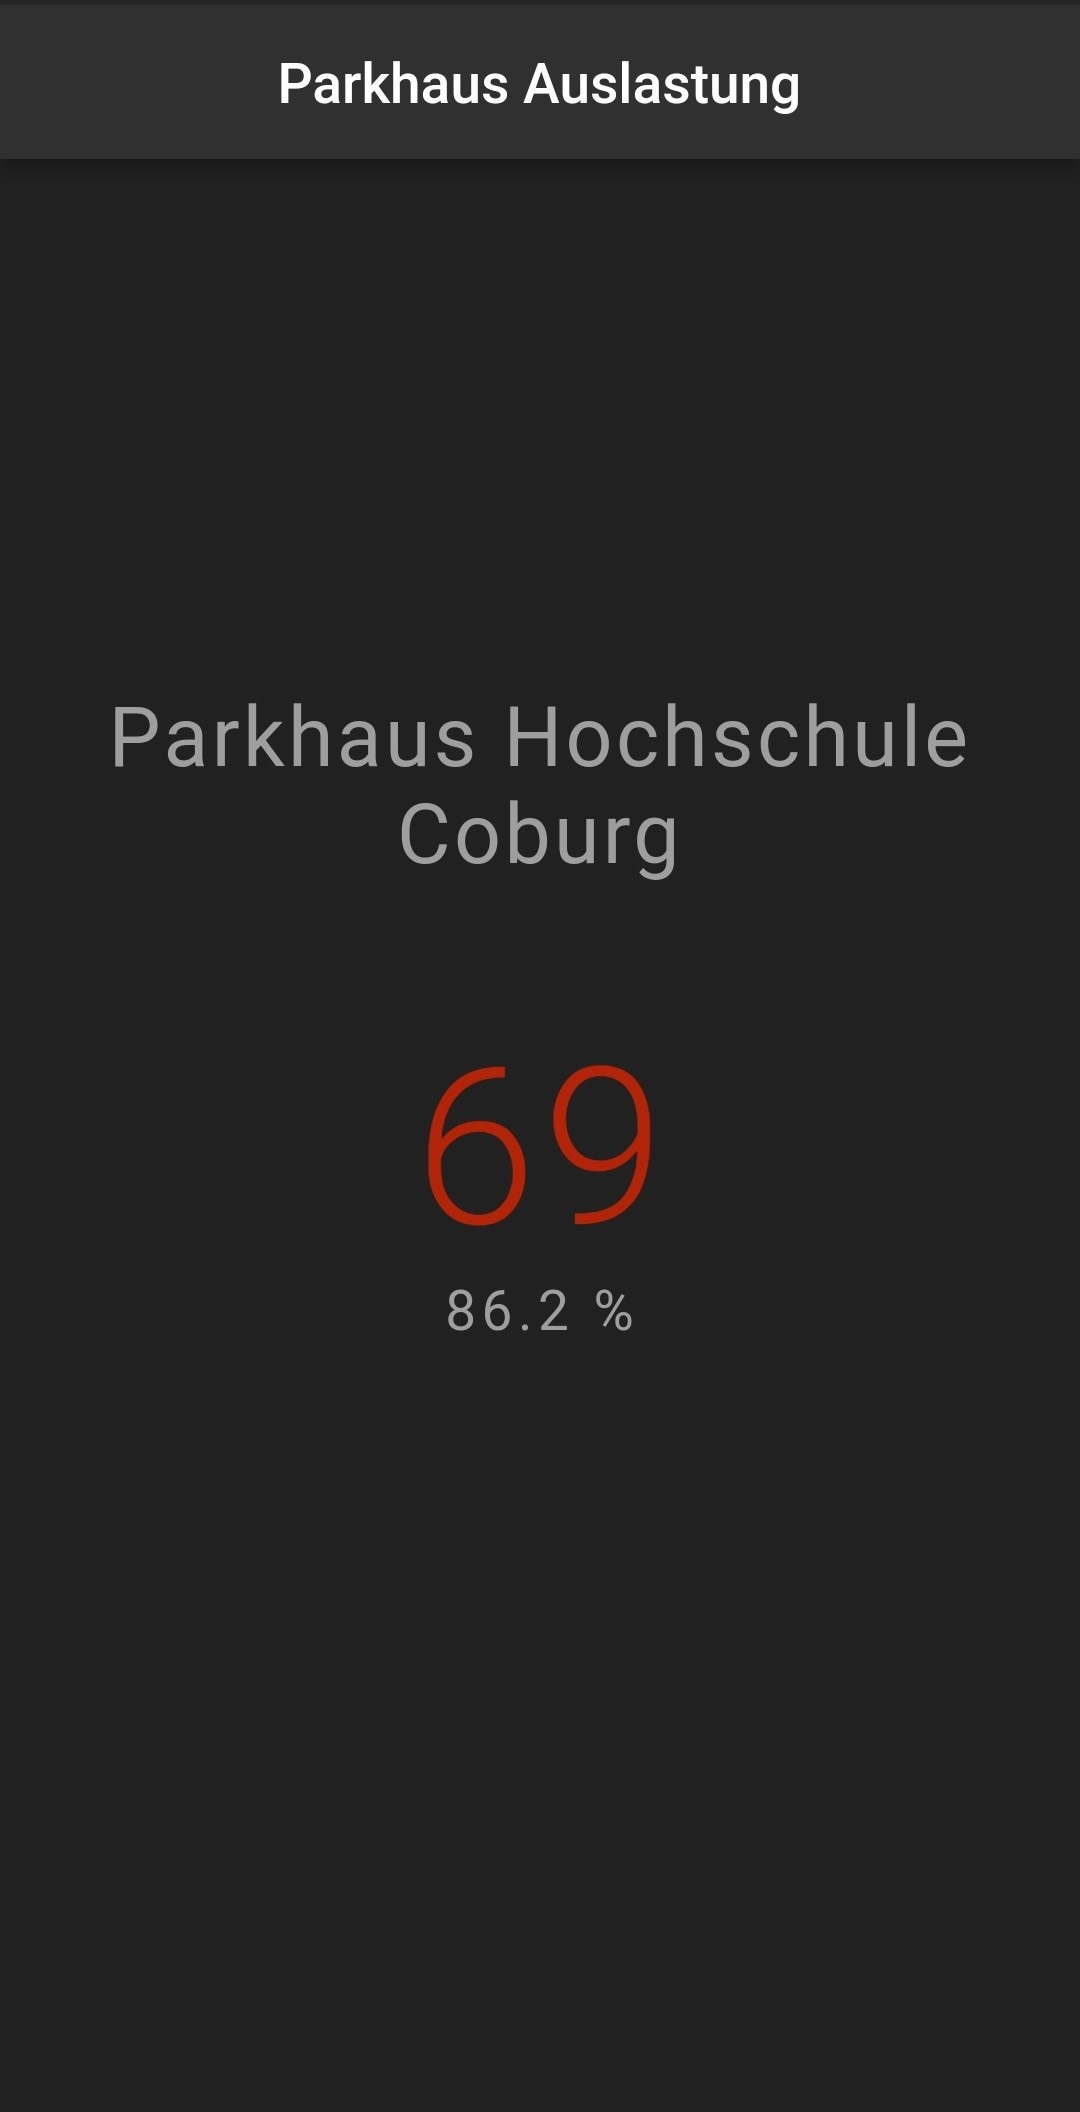
\includegraphics[width=0.3\myImageWidth]{Bilder/app_69.jpg}}
	\hfill
	\subfloat{
		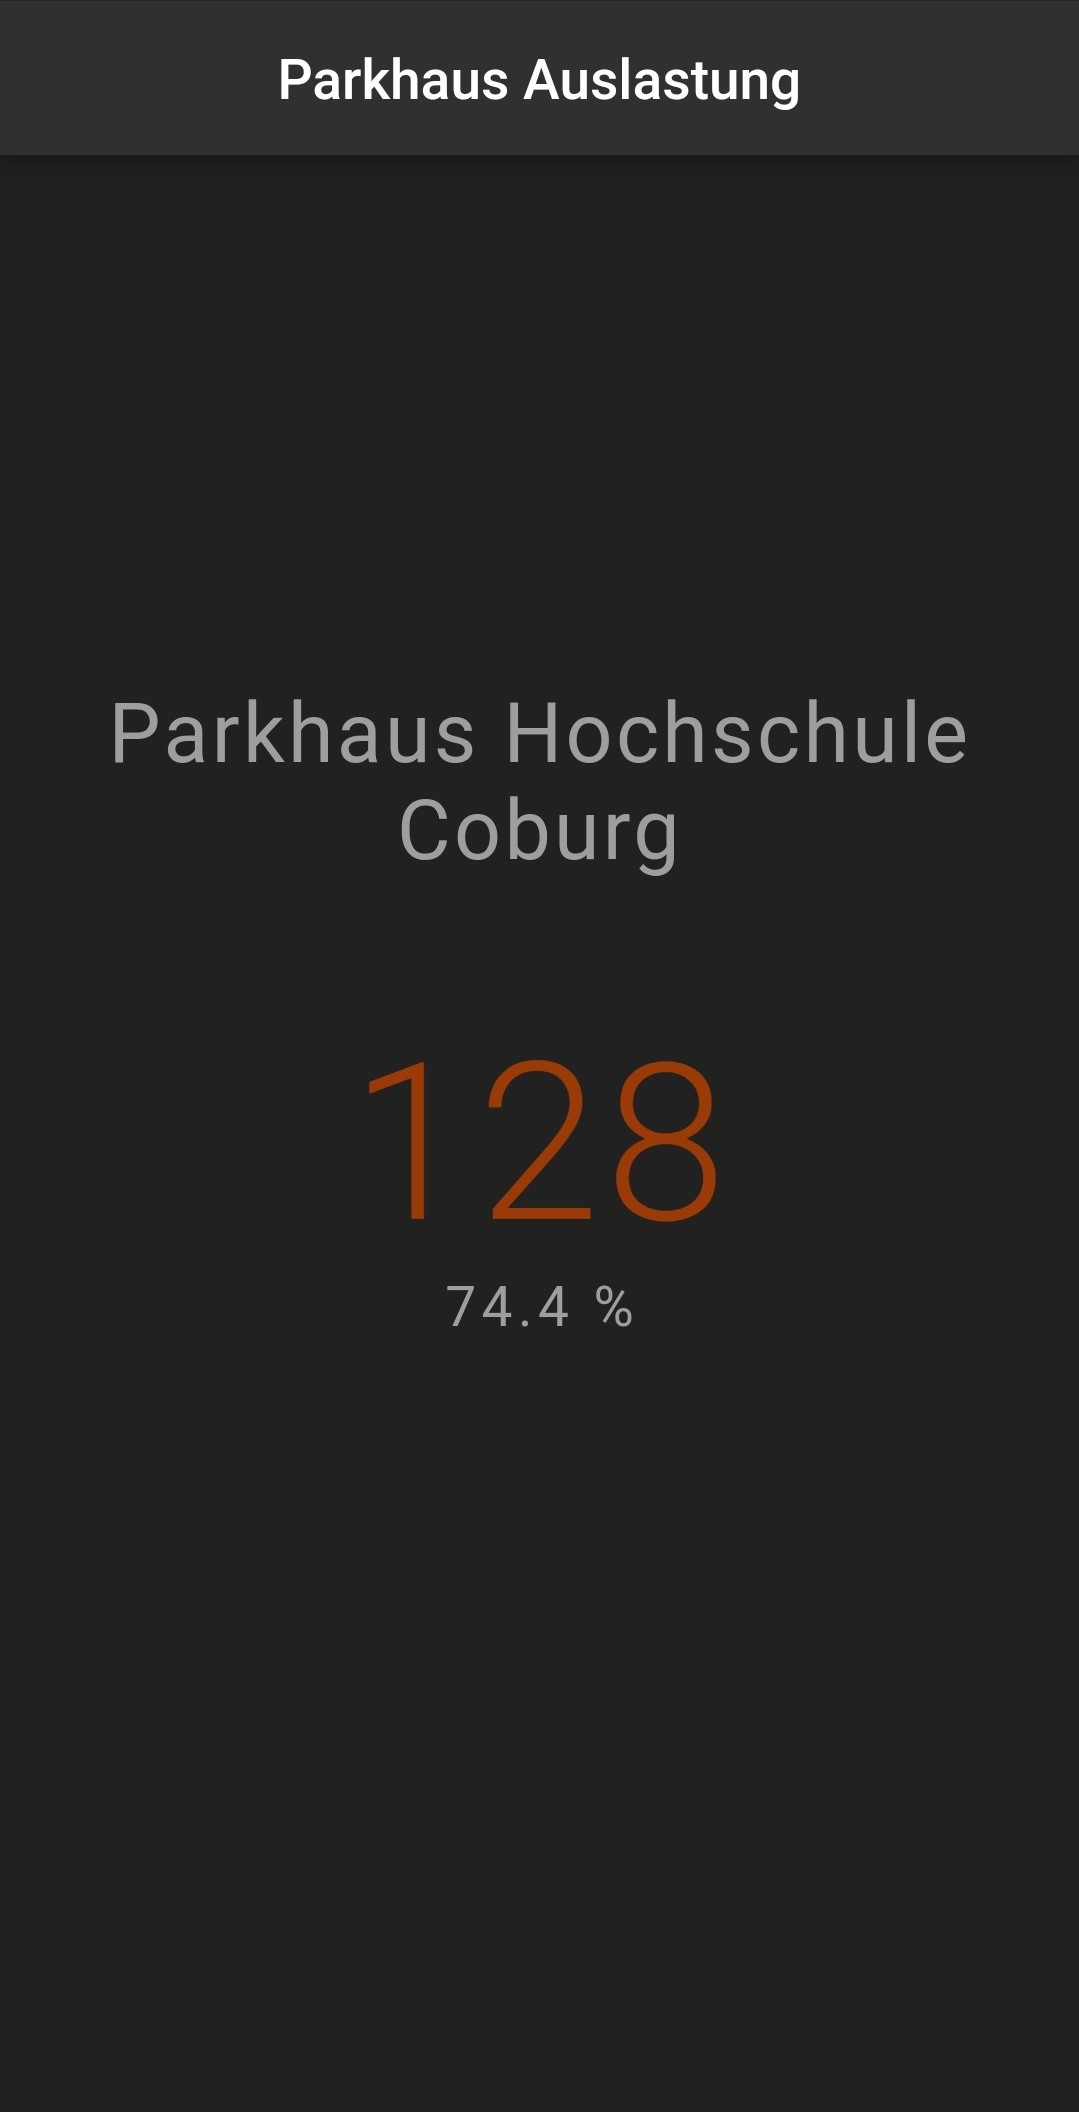
\includegraphics[width=0.3\myImageWidth]{Bilder/app_128.jpg}}
	\hfill
	\subfloat{
		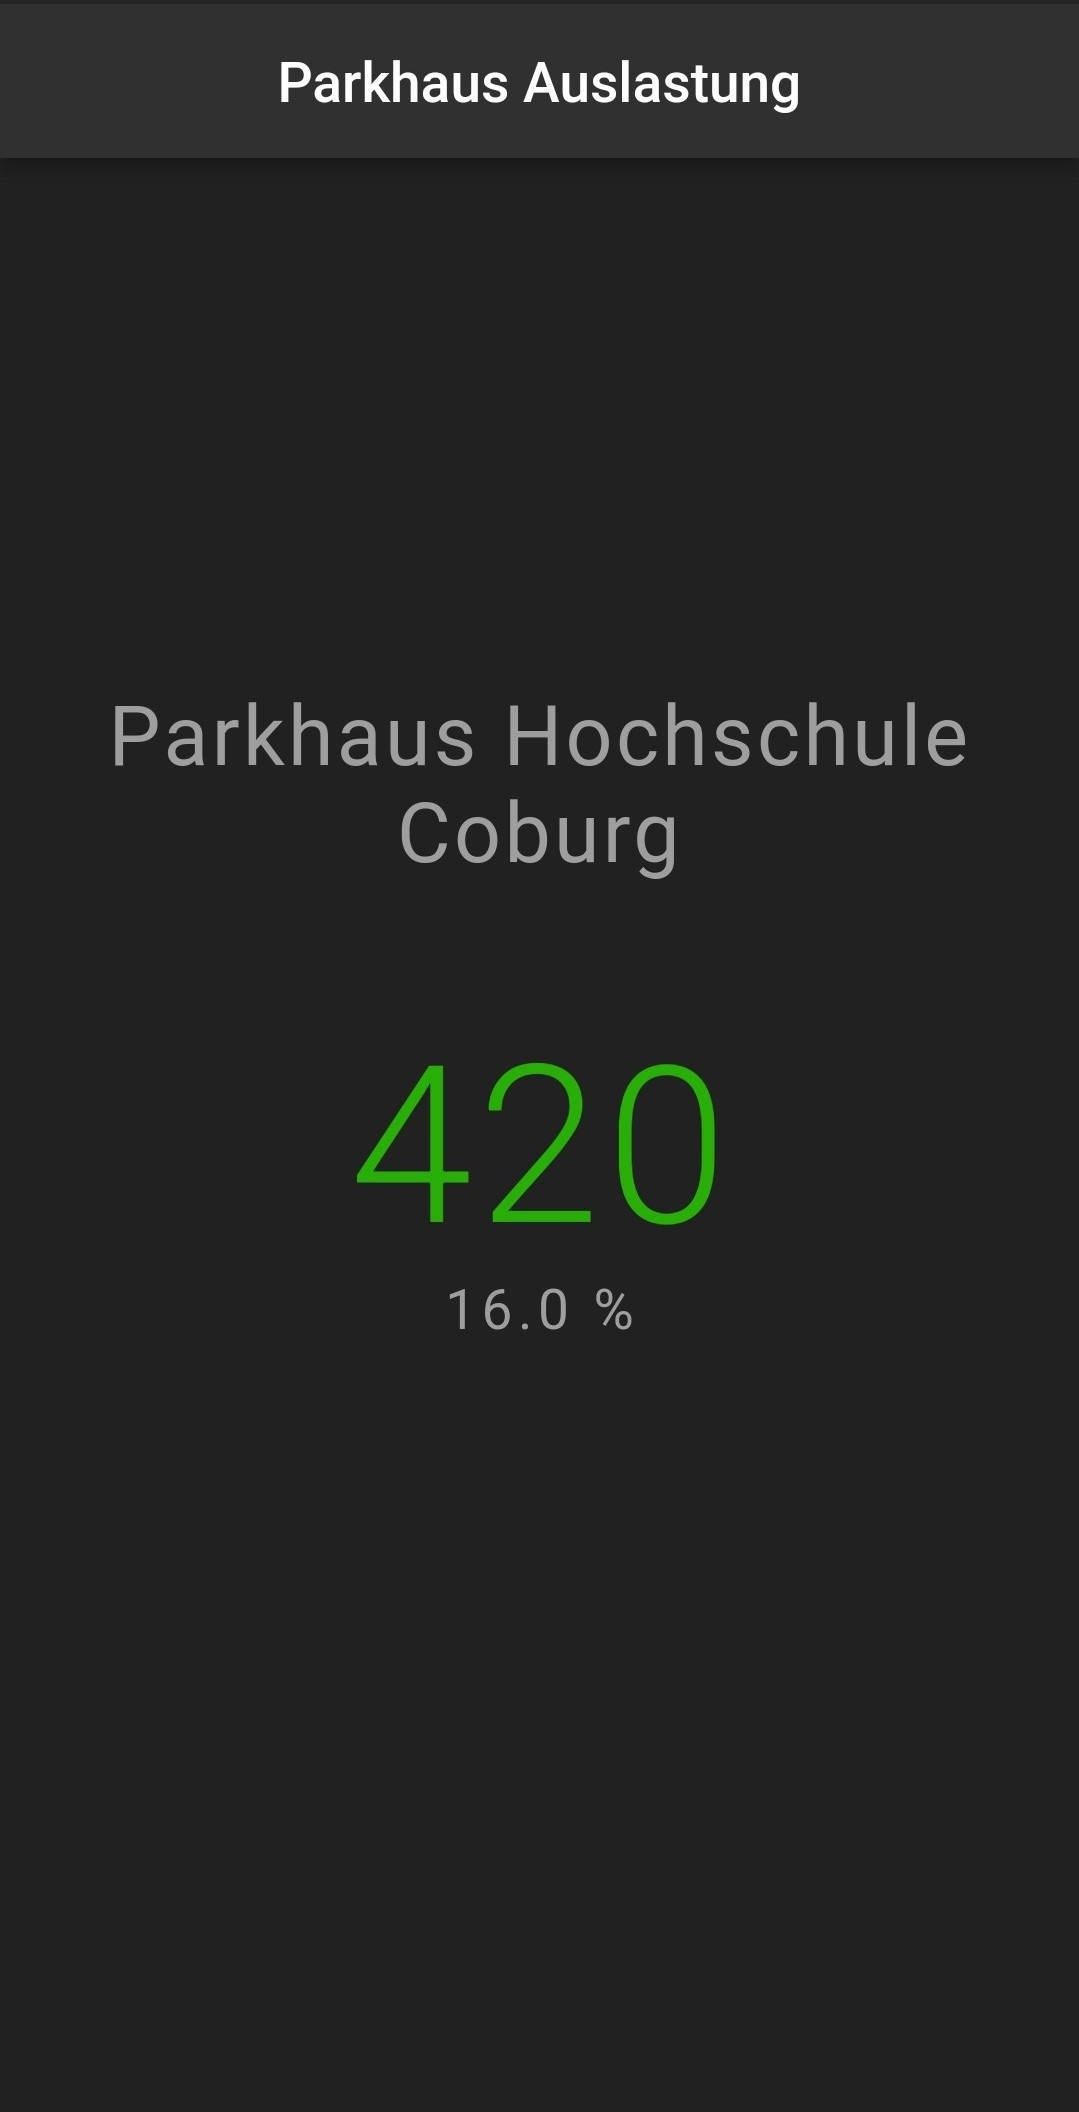
\includegraphics[width=0.3\myImageWidth]{Bilder/app_420.jpg}}
	\caption[Screenshots der App]{Screenshots der App (Quelle: eigene Darstellung)}\label{fig:app}
\end{figure}

Flutter und Dart stellen ein leistungsstarkes Framework und eine Programmiersprache dar, die von Google entwickelt wurden, um die Entwicklung plattformübergreifender Apps zu vereinfachen.
Flutter ermöglicht die Erstellung reaktiver Benutzeroberflächen, während Dart eine effiziente und objektorientierte Programmierung unterstützt.
Die Verwendung einer einzigen Codebasis für verschiedene Plattformen verbessert die Wartung und Skalierbarkeit der App erheblich.~\cite{awsWasIstFlutter}~\cite{dartDartOverview}

Wie bereits genannt, dient MQTT als leichtgewichtiges und zuverlässiges Kommunikationsprotokoll zum Empfangen der Nachrichten.
Die App abonniert die Topic des entsprechenden Parkplatzes beim Broker, um diese Informationen anzuzeigen.
Im aktuellen Prototypen ist die Topic hartkodiert.
